%%%%%%%%%%%%%%%%%%%%%%%%%%%%%%%%%%%%%%%%%
% Short Sectioned Assignment
% LaTeX Template
% Version 1.0 (5/5/12)
%
% This template has been downloaded from:
% http://www.LaTeXTemplates.com
%
% Original author:
% Frits Wenneker (http://www.howtotex.com)
%
% License:
% CC BY-NC-SA 3.0 (http://creativecommons.org/licenses/by-nc-sa/3.0/)
%
%%%%%%%%%%%%%%%%%%%%%%%%%%%%%%%%%%%%%%%%%

%----------------------------------------------------------------------------------------
%	PACKAGES AND OTHER DOCUMENT CONFIGURATIONS
%----------------------------------------------------------------------------------------

\documentclass[paper=a4, fontsize=9pt]{scrartcl} % A4 paper and 11pt font size


\usepackage[T1]{fontenc} % Use 8-bit encoding that has 256 glyphs
\usepackage[english,francais]{babel} % Français et anglais
\usepackage[utf8]{inputenc} 

\usepackage{amsmath,amsfonts,amsthm} % Math packages

\usepackage{enumitem}
\usepackage{lmodern}
\usepackage{url}
\usepackage{eurosym} % signe Euros
\usepackage{geometry} % Pour passer au format A4
\geometry{a4paper} % 
\usepackage{graphicx} % Required for including pictures
\usepackage{float} % Allows putting an [H] in \begin{figure} to specify the exact location of the figure

\usepackage{multicol}

\usepackage{verbatim}

\usepackage{sectsty} % Allows customizing section commands
\allsectionsfont{\centering \normalfont\scshape} % Make all sections centered, the default font and small caps

%----------------------------------------------------------------------------------------
%	Pied de Page
%----------------------------------------------------------------------------------------


\usepackage{fancyhdr} % Custom headers and footers
\pagestyle{fancyplain} % Makes all pages in the document conform to the custom headers and footers
\fancyhead{} % No page header - if you want one, create it in the same way as the footers below
\fancyfoot[C]{Triangles} % Empty center footer
\fancyfoot[R]{\thepage} % Page numbering for right footer

\renewcommand{\headrulewidth}{0pt} % Remove header underlines
\renewcommand{\footrulewidth}{0pt} % Remove footer underlines

%\usepackage{titling}
%\setlength{\droptitle}{-2.5cm}
%\setlength{\headheight}{13.6pt} % Customize the height of the header

\setlength\parindent{0pt} % Removes all indentation from paragraphs - comment this line for an assignment with lots of text


%----------------------------------------------------------------------------------------
%	Titre
%----------------------------------------------------------------------------------------

\newcommand{\horrule}[1]{\rule{\linewidth}{#1}} % Create horizontal rule command with 1 argument of height


\title{	
  \vspace{-10ex}
  \horrule{0.5pt} \\[0.4cm] % Thin top horizontal rule
  \huge Pythagore\\ % The assignment title
  \horrule{2pt} \\[0.5cm] % Thick bottom horizontal rule
}

\author{}
\date{\vspace{-10ex}} % Today's date or a custom date

%----------------------------------------------------------------------------------------
%	Début du document
%----------------------------------------------------------------------------------------

\begin{document}

%----------------------------------------------------------------------------------------
% RE-DEFINITION
%----------------------------------------------------------------------------------------
% MATHS
%-----------

\newtheorem{Definition}{Définition}
\newtheorem{Theorem}{Théorème}
\newtheorem{Proposition}{Propriété}

% MATHS
%-----------
\renewcommand{\labelitemi}{$\bullet$}
\renewcommand{\labelitemii}{$\circ$}
%----------------------------------------------------------------------------------------
%	Titre
%----------------------------------------------------------------------------------------

\maketitle % Print the title
\setlength{\columnseprule}{1pt}

\begin{multicols}{2}

\section{Un nombre au carré}


  \begin{Definition}
    Lorsqu'on multiplie un nombre par lui-même, on parle de nombre \textbf{au carré}.\\
    $8^2 = 8 \times 8 = 64$
  \end{Definition}

  \paragraph{Vocabulaire}~~\\
  \textit{En plus de huit au carré pour $8^2$, on peut également dire :}
  \begin{itemize}	
  \item huit à la puissance 2
  \item huit exposant 2.
  \end{itemize}
  
  \paragraph{Calculette}~~\\
  \begin{itemize}	
  \item On utilise la touche $x^2$.
  \end{itemize}


 \subsection{Le carré en géométrie}
 
 \begin{Definition}
	Un carré est un quadrilatère dont les côtés sont de mêmes longueurs et avec 4 angles droits.\\
	\textbf{Aire} : $5^2$\\
	\textbf{Périmètre} : $4 \times 5$
\end{Definition}

	\begin{figure}[H]
	  \centering
	  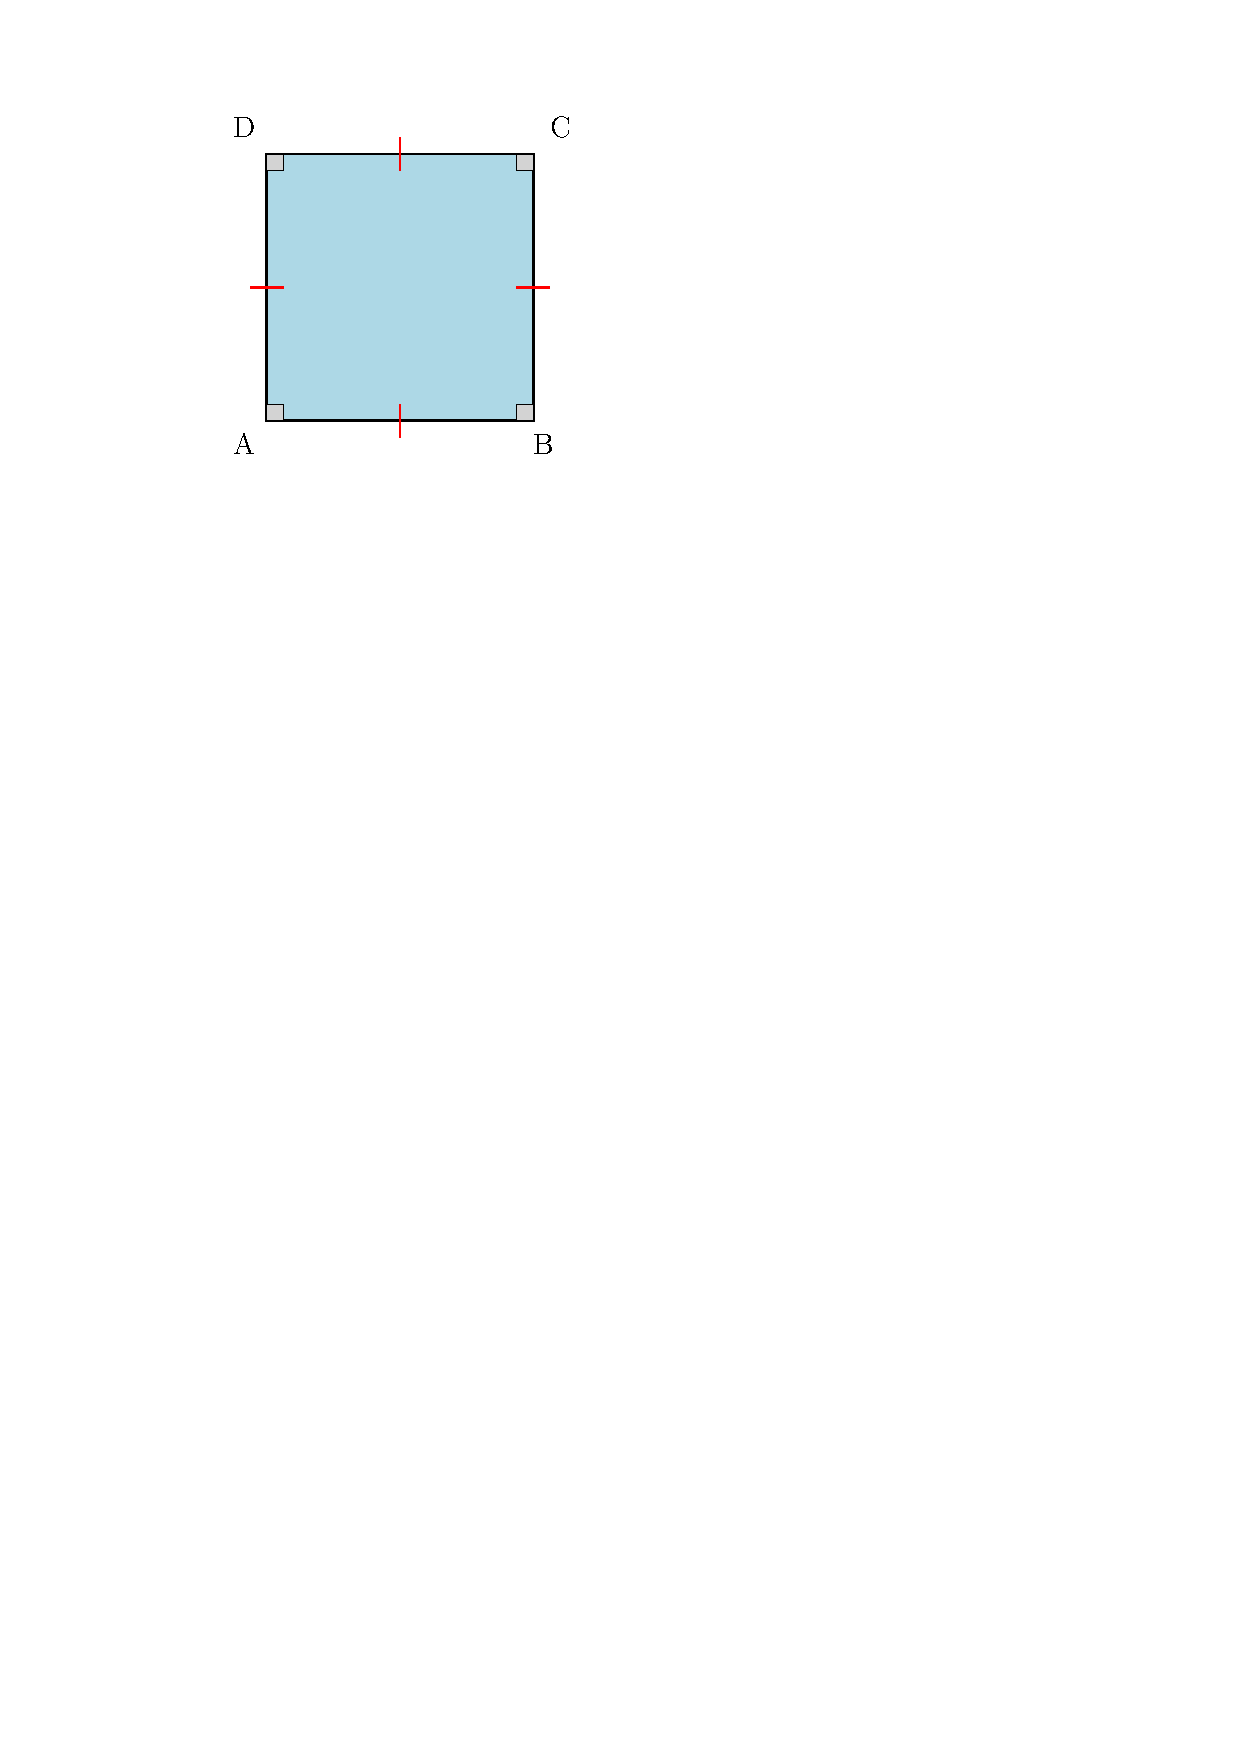
\includegraphics[width=0.6\linewidth]{sources/1/carre.pdf}
	\end{figure}

\end{multicols}

\begin{multicols}{2}

\section{Caractérisation du triangle rectangle}


\begin{Theorem}{1) Propriété de Pythagore}
    Dans un triangle \textbf{rectangle}, le carré de l’hypoténuse est égal à la somme des carrés des autres 
côtés.
 \end{Theorem}

  \begin{Proposition}{Énoncé exercice}

    Soit un triangle ABC rectangle en B. 
	$$AB^2 + BC^2 = AC^2$$

	\begin{figure}[H]
	  \centering
	  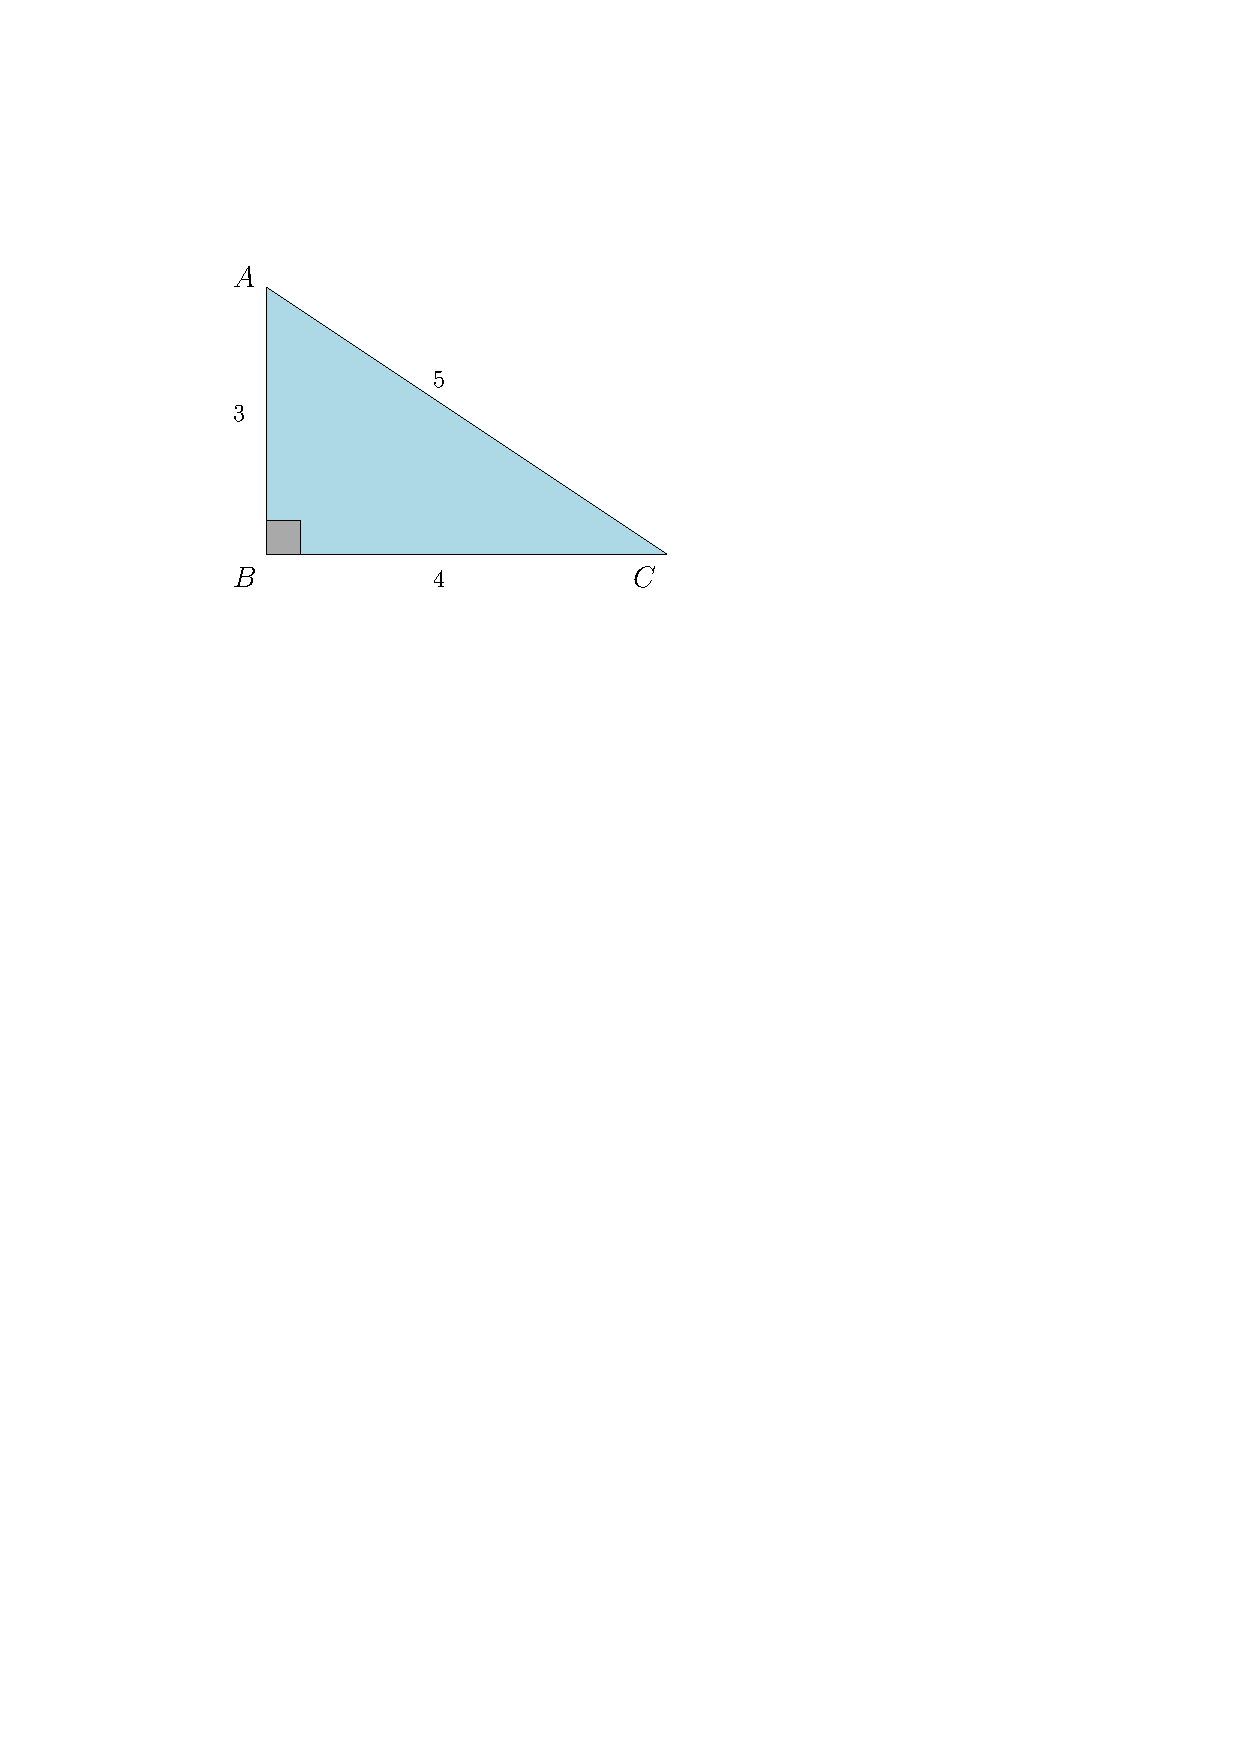
\includegraphics[width=\linewidth]{sources/1/tri-pytha.pdf}
	\end{figure}
\end{Proposition}

\end{multicols}

\begin{multicols}{2}

\section{Racine carré d'un nombre}

  \begin{Definition}
    Le nombre qui, mis au carré donne 25 s’appelle \textbf{la racine carrée} de 25. On le note $\sqrt{25} = 5$ car $5^2 = 25$.
  \end{Definition}

  \paragraph{Vocabulaire}~~\\
  \textit{On dit racine de 121.}

  \paragraph{Calculette}~~\\
  On utilise la touche $\sqrt{x}$.\\
  Attention $\sqrt{2 + 5} \neq \sqrt{2} + \sqrt{5}$
  

	\paragraph{Attention aux calculs}~~\\

    \begin{itemize}
    \item $\sqrt{2 + 5} = $
    \item $\sqrt{2} + \sqrt{5}= $
    \item $\sqrt{-4} = $
   \end{itemize}


  \section{Utilisations du théorème de Pythagore}
    
    \begin{itemize}	
    \item Prouver qu'un triangle est rectangle
    \item Prouver qu'un triangle n'est pas rectangle. 
    \item Calculer la troisième longueur d'un triangle rectangle à l'aide de la racine carré.
    \end{itemize}
  
\end{multicols}

\end{document}
